\chapter{I protocolli per l'IoT}
Parallelamente agli sviluppi tecnologici nel mondo dell'elettronica si è posto il problema di trovare protocolli di comunicazione adeguati che potessero permettere agli smart objects di comunicare tra loro e verso interfacce di più alto livello, rispettando le limitazioni imposte da una spesso ridotta capacità computazionale o di autonomia energetica.


\section{Il livello Data Link}
In questo paragrafo saranno trattati i protocolli del livello Data Link applicati all'IoT. Grandi protagonisti in questo ambito sono i protocolli radio, data la natura indipendente e mobile degli smart objects, che permettono ai dispositivi di comunicare senza avere necessità di collegamenti ingombranti e poco utili. Le frequenze trasmissive sono solitamente quelle ISM (Industrial, Scientific and Medical), porzioni dello spettro elettromagnetico non commerciali e che possono essere liberamente utilizzate, rispettando le potenze trasmissive imposte dai singoli Paesi. Troviamo quindi spesso protocolli che utilizzano le frequenze intorno ai 2,4 GHz come 802.15.4, WiFi (nei suoi standard b/g), Bluetooth, ANT+ ecc...
\\Queste frequenze garantiscono una discreta immunità da interferenze, la possibilità di utilizzare antenne ridotte e una buona larghezza di banda, anche se una scarsa penetrabilità degli ostacoli, il che limita solitamente il raggio utile a non più di 100 metri, a seconda della modulazione utilizzata.
\\\\Proprio per via dello scarso raggio d'azione ultimamente si stanno affacciando anche protocolli che operano nelle frequenze Sub-GHz, ovvero al di sotto del GHz, solitamente sfruttando le frequenze 868-915 MHz. L'utilizzo di frequenze più ridotte permette di trasmettere segnali ad una distanza maggiore, anche fino a 500-1000 Km, mantenendo pressochè uguali le potenze di trasmissione ma sacrificando il data rate. Alcuni network operativi sulle frequenze Sub-1GHz stanno nascendo per dare la possibilità agli smart objects di connettersi direttamente alla rete Internet senza bisogno di infrastrutture di supporto. Tra questi ricordiamo i più importanti, LoRa e SigFox, di cui parleremo successivamente.

\subsection{802.15.4 e ZigBee}
Tra i protocolli radio che maggiormente hanno trovato successo nel mondo IoT sicuramente 802.15.4, e le sue commercializzazioni, è uno di quelli che spicca maggiormente. Come tutte le reti appartenenti alle specifiche IEEE 802.15.x si tratta di un protocollo sviluppato per reti wireless a stretto raggio di copertura del segnale e con basse velocità di trasferimento, ovvero reti LR-WPAN (Low Rate Wireless Personal Area Network).
\\In questo ambito le applicazioni che vogliono utilizzare queste specifiche hanno richieste di:
\begin{itemize}
\item Bassi costi
\item Bassa complessità di implementazione
\item Scarsi consumi energetici, ovvero ampia durata di eventuali batterie
\item Data rate modesti
\end{itemize}
Le topologie di rete previste in questo standard sono due, a stella e peer-to-peer, e con due differenti tipologie di dispositivi partecipanti: Full Function Device (FFD) e Reduced Function Device (RFD). Gli RFD sono tipicamente dispositivi a scarsa o scarsissima potenza computazionale che sono in grado di svolgere funzioni basiche e pertanto possono comunicare solamente con dispositivi FFD, i quali si occuperanno, se necessario, di smistare i messaggi verso altri RFD o verso dispositivi di più alto livello.
\\Nella topologia a stella troviamo un nodo FDD centrale che funge da \textit{PAN Coordinator}, ovvero smista i pacchetti provenienti dai nodi RFD e comunica con altri nodi FDD che però non hanno ruolo di coordinatori. In questa topologia è il \textit{Coordinator} che per primo comunica agli altri nodi l'identificativo della rete, rendendo la rete completamente indipendente da eventuali altre reti presenti.
\\Nella topologia peer-to-peer, invece, il primo device FDD che trasmette diventa \textit{Coordinator} ma in qualunque momento un nodo FDD può assumere quel ruolo per coordinare nodi RFD che sono collegati a lui e instradare il messaggio sulla rete. 802.15.4 non definisce alcun protocollo di routing per questa topologia di rete, demandando il compito agli strati superiori.
\\\\La modalità di accesso al canale è CSMA/CA (in versione "semplificata"), mentre per la trasmissione si utilizzano tecnologie \textit{Spread Spectrum} per ridurre le interferenze.
\\Le frequenze solitamente utilizzate sono le classiche 2.4 GHz, ma in realtà talvolta 802.15.4 viene utilizzato su frequenze Sub-1Ghz, in particolare 868 e 915 MHz e, con le ultime revisioni dello standard, è stata introdotta anche la possibilità di utilizzare frequenze a 5 GHz, molto più libere da interferenze.
\\I data-rates supportati sono 250, 40 e 20 kb/s e il raggio utile di trasmissione non supera i 30-40 metri.
\\\\Il pacchetto 802.15.4, a livello PHY (\textit{Physical}) è formato da:
\begin{itemize}
\item \textbf{Preamble}: 4 byte di lunghezza, utilizzato per la sincronizzazione
\item \textbf{Start of Packet Delimiter}: 8 bit di lunghezza, utilizzato anche questo per sincronizzare la comunicazione
\item \textbf{PHY Header}: 1 byte, contenente il campo \textit{Frame Length} di 7 bit più 1 bit riservato per usi futuri.
\item \textbf{PHY Service Data Unit (PSDU)}: da 0 a 127 byte di lunghezza, contenente a sua volta il pacchetto MAC.
\end{itemize}
Il pacchetto dello strato MAC è articolato ma è interessante notare come l'indirizzamento preveda un indirizzo univoco da 64 bit per ogni dispositivo sulla stessa rete PAN e quindi, potenzialmente, circa 18 trilioni di dispositivi per ogni network.
\\Tuttavia al momento dell'associazione alla rete il \textit{Coordinator} assegna al device uno \textit{short-address} da 16 bit, limitando quindi l'indirizzamento a 65'535 dispositivi, numero comunque sufficiente a coprire ampiamente le esigenze odierne.
\begin{figure}[!h]
\centering
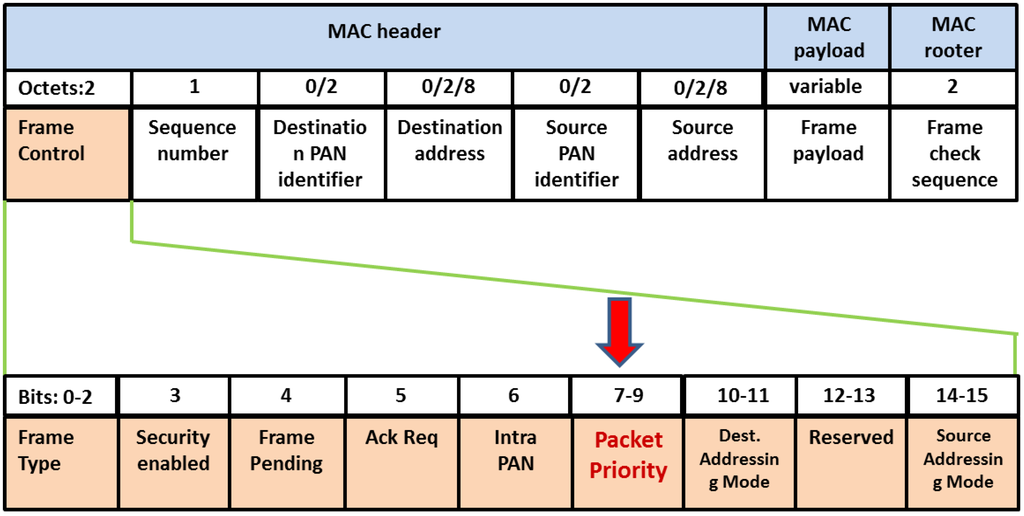
\includegraphics[scale=3.00]{immagini/802154-frame.png}
\caption{\textit{Il frame 802.15.4, sia a livello fisico che a livello MAC}}
\end{figure}
802.15.4 è in grando inoltre di sfruttare tecniche di accesso al canale e trasmissione/ricezione sincronizzate per ottimizzare al massimo il risparmio energetico, importante richiesta di questa tipologia di dispositivi, e prevede dei meccanismi di sicurezza integrati nello strato MAC, per fornire integrità, autenticazione e confidenzialità ai messaggi, pur mantenedo un basso profilo energetico.
\vspace{1.0cm}
\\Sopra lo standard 802.15.4 sono state costruite diverse "commercializzazioni" e standard operanti sui livelli più alti dello stack ISO/OSI. Uno dei più famosi e largamente utilizzati è certamente \textbf{ZigBee}, nato nel 2004 e giunto ora alla sua terza specifica. ZigBee prevede tre possibili tipologie di dispositivi partecipanti:
\begin{itemize}
\item \textit{ZigBee Coordinator}: coincide in tutto e per tutto con l'omonimo ruolo della specifica 802.15.4, ovvero si occupa di "creare" la rete, memorizzare eventuali chiavi di sicurezza e può operare da ponte tra più reti. Ci può essere un solo \textit{Coordinator} per ogni rete.
\item \textit{ZigBee Router}: questa tipologia di dispositivi permette di scambiare pacchetti tra i dispositivi o tra porzioni della stessa rete, effettuando anche multi-hopping, ovvero ritrasmissione e routing.
\item \textit{ZigBee End Device}: sono i dispositivi a funzionalità minime, possono dialogare solo con i \textit{Coordinator} o con i \textit{Router} e non partecipano al multi-hop di un messaggio.
\end{itemize}
Il protocollo di routing solitamente utilizzato è l'AODV (\textit{Ad-hoc On-demand Distance Vector}, un algoritmo derivato dal classico \textit{Distance Vector} ma pensato per reti mobili e dove le trasmissioni devono essere limitate al minimo. AODV, a differenza di Distance Vector classico, interviene a calcolare il percorso di routing solo quando richiesto, ovvero quando si cerca di accedere ad un nodo di cui ancora non si conosce il percorso; questo limita notevolmente il traffico per percorsi già stabiliti anche se aumenta considerevolmente il tempo di risposta nel caso il routing sia ancora sconosciuto. AODV supporta anche instradamenti di tipo unicast e multicast.
\\\\Altro neonato protocollo che si basa su 802.15.4 è \textbf{Thread}, protocollo nato nei laboratori di ricerca di Nest (ora proprietà di Google) ma supportato anche da altre grandi aziende come Samsung e NXP Semicondutors.

\subsection{Altri}
Diversi altri protocolli hanno affermato la propria importanza nel mondo IoT negli ultimi anni, differenziandosi in maniera abbastanza netta a seconda della tipologia d'uso del dispositivo che si va a sviluppare.
\\Sempre nell'ambito radio è impossibile non citare \textbf{Bluetooth Low Energy} (BLE), nato sotto il nome di \textit{WiBree} diventando poi \textit{Bluetooth Smart} per il pubblico, proposto all'interno della specifica Bluetooth 4.0 nel 2010. BLE viene pensato per sopperire alla mancanza di profili Bluetooth adatti agli smart objects e in generale adatti ai dispositivi funzionanti a batteria, profili che non necessitano di trasferire grandi quantità di dati.
\\BLE, come tutta la tecnologia Bluetooth, sfrutta le frequenze 2.4 GHz ma a differenza delle altre modalità utilizza modulazioni d'onda differenti, per mantenere bassi i consumi energetici. La specifica BLE è stata pensata fin da subito con uno sguardo alla sicurezza, implementando a livello MAC delle tecniche di criptazione, alcune delle quali basate su AES a 128 bit con CBC-MAC, per garantire confidenzialità e autenticazione più altri algoritmi di Message Integrity Check.\\Le topologie di rete permesse da BLE sono le classiche di Bluetooth, ovvero scatternet, anche se ultimamente sono nate librerie di livello applicativo che permettono con successo di instaurare reti di tipo mesh (peer-to-peer). \\Sebbene BLE fosse solo una parte di Bluetooth 4, in quanto la specifica prevedeva anche una modalità High Speed (simile a quella presente in Bluetooth 3.0) in grado di trasferire dati a velocità intorno ai 25 Mb/s e la classica modalità a profili, venne recepita come unica vera novità del nuovo standard ed ebbe un successo enorme. Molto presto i maggiori produttori di semiconduttori svilupparono chip "single-mode", ovvero con il solo stack BLE., che permetteva di utilizzare microcontrollori a ridotta capacità e quindi abbattere costi e consumi. Il mercato rispose bene a questi prodotti, tanto che, per esempio, Nordic Semiconductors ha costruito il proprio core-business su SoC (System on Chip) BLE, sfruttando le proprie già ampie conoscenze nelle modulazioni delle frequenze 2.4 GHz. \\Altri grandi produttori, come STMicroelectronics, Texas Instruments, NXP Semiconductors, CSR ed altri, hanno fatto fortuna grazie a BLE e grazie spesso a sapienti accoppiate, in un unico chip, di questo standard con altre affermate tecnologie del mondo IoT.
\\\\Altra interessante famiglia di tecnologie radio è sicuramente quella Sub-1GHz che negli ultimissimi anni sta aumentando la propria visibilità anche al pubblico. Tra queste le più note sono certamente LoRaWAN e SigFox, tecnologie LPWAN (Low Power Wide Area Network) che sfruttano le bande sotto il GHz di frequenze per il traffico radio, con una particolare modulazione chiamata Ultra-narrow band, che permette di trasmettere a distanze elevatissime, anche decine di Km, utilizzando pochissima potenza di trasmissione. In maniera speculare i dispositivi riceventi sono in grado di captare i segnali trasmessi con questa modulazione anche se questi sono deboli, senza quindi necessitare di antenne ingombranti.
\\La modulazione Ultra-narrow Band non è nuova, tanto che veniva utilizzata dai sommergibili americani per comunicare già nella Prima Guerra Mondiale, ma è stata ripresa ed adattata per creare network a ridottissima banda passante (si parla di un massimo di 12 byte per messaggio su rete SigFox, mentre LoRaWAN ha una banda passante di circa 22 Kb/s) ma che sono in grado di coprire grosse aree geografiche a costi ridotti.
\\L'idea è infatti quella di utilizzare apparati trasmissivi già esistenti, tipo torri televisive, radiofoniche o celle telefoniche, per installare ripetitori in grado di creare una rete specifica per l'IoT e fornire agli smart objects la possibilità di entrare direttamente sulla rete Internet, senza passare attraverso apparati intermedi.
\\Entrambe le tecnologie stanno sempre più prendendo piede, anche grazie ad accordi con operatori di telecomunicazioni e permetteranno un'indipendenza ai dispositivi smart che oggi solo tecnologie energeticamente (ed economicamente) costose come 2G/3G/4G possono dare.
\\\\Anche le tecnologie 3GPP per la telefonia mobile, come GSM/GPRS, CDMA, UMTS e LTE hanno un certo rilievo nel mondo IoT perchè permettono l'accesso ad Internet praticamente in ogni paese del Mondo, dove i Paesi maggiormente industrializzati hanno coperture di telefonia mobile quasi prossime al 100\%. Tuttavia le reti Sub-GHz potrebbero ricoprire presto questo ruolo, essendo maggiormente efficienti da un punto di vista energetico, restrizione non opzionale nel campo degli smart objects.
\\\\Altre tecnologie, come quelle radio a cortissimo raggio, tipo NFC, o come quelle cablate, come Ethernet, ricoprono ruoli più marginali e sono meno utilizzate per la comunicazione interdevices, perchè non sono in grado di rispondere pienamente ai requisiti imposti dalla tipologia di utilizzo di questi dispositivi.

\section{I livelli di rete e trasporto}
Nel momento in cui nasceva l'IoT la rete Internet era oramai divenuta una tecnologia solida e largamente utilizzata, e il suo attore protagonista era certamente il protocollo IP. Fu lecito quindi domandarsi se IP fosse adatto anche per le comunicazioni tra questi device, dotati spesso di capacità computazionali e memorie ridottissime in confronti ai sempre più potenti calcolatori che si affacciavano sul mercato tecnologico mondiale.
\\I requisiti di una rete di smart objects erano principalmente:
\begin{itemize}
\item Evolvibilità: le reti di smart objects devono essere in grado di cambiare, anche radicalmente, i propri obiettivi e i propri requisiti senza che ci fosse necessità di riprogettare la rete.
\item Scalabilità: potenzialmente le reti di smart objects hanno migliaia e migliaia di nodi e la rete deve essere in grado non solo di sopportare il traffico generato, ma anche di rimapparsi velocemente in caso di connessione/disconnessione di un nodo.
\item Diversità di applicazioni e tecnologia: i nodi di queste reti sono potenzialmente tutti differenti, sia per tecnologie che per applicazioni, e il protocollo alla base di questa rete deve essere flessibile al punto da permettere a tutti i tipi di nodi di entrare in comunicazione con gli altri.
\item Interoperabilità: requisito molto importante, gli smart objects non devono solo essere in grado di comunicare tra loro, ma anche verso reti e dispositivi già esistenti su reti differenti.
\item Bassi costi e consumi: come sempre, costi e consumi energetici sono un aspetto fondamentale nella determinazione delle tecnologie applicabili all'IoT e anche i protocolli di rete non possono trascurare questi importanti requisiti.
\end{itemize}

\subsection{IPv6 e lo strato 6LoWPAN}
IP era l'unico protocollo in grado di rispondere perfettamente a tutti i requisiti richiesti ma a questo punto venne spontaneo chiedersi se fosse più saggio utilizzare IPv4, consolidato nel mondo dei calcolatori, oppure il neonato IPv6, ancora "acerbo" ma promettente e sicuro successore della versione v4 in un futuro non troppo remoto.
\\Fu chiaro fin da subito che lo spazio di indirizzamento di IPv4, che utilizza 32 bit per gli indirizzi, era troppo ristretto per poter sostenere reti potenzialmente numerosissime di smart objects e quindi la scelta ricadde su IPv6, principalmente per questo motivo ma anche per via di altre ragioni come la possibilità di effettuare routing multicast o il supporto integrato alla sicurezza delle comunicazioni.
\\Nacque addirittura una organizzazione non-profit per sostenere l'utilizzo di IP, e in particolare della sua versione IPv6, nelle comunicazioni tra smart objects, la IPSO Alliance (IP for Smart Objects), sostenuta anche da grandi enti di standardizzazione come IETF, IEEE ed ETSI.
\\\\Alcuni standard radio erano già direttamente compatibili con il protocollo IPv6, altri necessitavano di adattamenti. Il più importante strato di adattamento è certamente \textbf{6LoWPAN} (IPv6 over Low power Wireless Personal Area Network), concepito da un gruppo di lavoro di IETF per portare connettività IPv6 sullo standard 802.15.4, sfruttando una particolare compressione dell'header e riducendo lo stack IPv6 al minimo indispensabile per essere in grado di funzionare su dispositivi con modeste capacità di calcolo e ridotta memoria.
\\6LoWPAN introduce anche alcune funzionalità di base necessarie alle reti di smart objects come il mesh networking e la neighbour discovery e utilizza protocolli di routing semplici ma funzionali, come RPL.
\\\\Anche gli standard Thread e ZigBee prevedono l'utilizzo di 6LoWPAN come strato intermedio per l'utilizzo di IPv6.

\subsection{TCP e UDP}
Entrambi i protocolli del livello di trasporto sono utilizzabili in reti IoT, ognuno con le sue caratteristiche. Inizialmente si pensò che UDP fosse il candidato migliore ad essere utilizzato per via di alcune sue caratteristiche che lo rendevano estremamente interessante: innanzitutto il basso overhead garantisce di occupare per un minor tempo il trasmettitore, dove, soprattutto se si tratta di canali radio, il risparmio di energia è mandatorio; non si ha un meccanismo di ritrasmissione dei pacchetti persi, ma in generale in applicazioni IoT questo non è un problema e inoltre UDP permette di effettuare con semplicità trasmissioni di tipo multicast o broadcast, senza necessità di instaurare alcun tipo di connessione.

\section{Il livello applicativo}

\subsection{CoAP}
\subsection{Altri}
